% !TeX program = pdflatex
% Standalone source. Compile with pdfLaTeX; no external figures are required.
\documentclass[11pt,a4paper]{article}
\usepackage[margin=20mm]{geometry}
\usepackage[T1]{fontenc}
\usepackage{lmodern}
\usepackage{amsmath,amssymb,booktabs,array,xcolor,tikz,fancyhdr,hyperref}
\usetikzlibrary{calc,arrows.meta}
\hypersetup{colorlinks=true,linkcolor=blue!50!black,urlcolor=blue!50!black}
\definecolor{accent}{HTML}{124E66}
\definecolor{pcol}{HTML}{A24021}
\definecolor{ncol}{HTML}{175A86}
\pagestyle{fancy}\fancyhf{}\fancyhead[L]{\small EE3032 / Fall 2024 / HW1}
\fancyhead[R]{\small CMOS logic}\fancyfoot[C]{\thepage}
\setlength{\headheight}{15pt}\setlength{\parindent}{0pt}\setlength{\parskip}{6pt}
\renewcommand{\arraystretch}{1.2}
\newcommand{\answer}[1]{\par\noindent\colorbox{accent!9}{\parbox{0.96\linewidth}{#1}}\par}
\newcommand{\AND}{\,}
\newcommand{\VDD}{V_{\mathrm{DD}}}
\newcommand{\VSS}{V_{\mathrm{SS}}}
% A conventional switch-level MOS symbol: continuous channel, insulated gate,
% and a gate bubble for pMOS. Bulk terminals are omitted, as explained below.
% Arguments: device id, x, y, gate literal, p or n. t/b are upper/lower terminals.
\newcommand{\MOS}[5]{
  \coordinate (#1) at (#2,#3);
  \coordinate (#1t) at ($(#1)+(0,.55)$);
  \coordinate (#1b) at ($(#1)+(0,-.55)$);
  \draw (#1t)--($(#1)+(0,.30)$)--($(#1)+(-.18,.30)$);
  \draw ($(#1)+(-.18,.34)$)--($(#1)+(-.18,-.34)$);
  \draw ($(#1)+(-.18,-.30)$)--($(#1)+(0,-.30)$)--(#1b);
  \draw ($(#1)+(-.35,.33)$)--($(#1)+(-.35,-.33)$);
  \def\type{#5}\def\ptype{p}
  \ifx\type\ptype
    \draw ($(#1)+(-.78,0)$)--($(#1)+(-.53,0)$);
    \draw ($(#1)+(-.465,0)$) circle (.065);
    \draw ($(#1)+(-.40,0)$)--($(#1)+(-.35,0)$);
  \else
    \draw ($(#1)+(-.78,0)$)--($(#1)+(-.35,0)$);
  \fi
  \node[anchor=east] at ($(#1)+(-.82,0)$) {$#4$};
  \node[anchor=west,font=\scriptsize] at ($(#1)+(.10,0)$) {#1};
}
% A transmission-gate instance; its two MOS devices are expanded on page 3.
\newcommand{\TG}[4]{
  \node[draw,rounded corners=1pt,minimum width=11mm,minimum height=6mm,
        fill=accent!5,font=\small] (#1) at (#2,#3) {$\mathrm{TG}_{#4}$};
}
\begin{document}
\begin{center}
{\LARGE\bfseries 2024 Homework 1}\\[4pt]
{\large Static CMOS, Data Selection, and XNOR}\\[4pt]
{\small Introduction to VLSI Design / EE3032}
\end{center}
\textbf{Method and notation.} The solutions are derived from the original assignment,
then compared with two user-supplied handwritten references. Here $+$ means OR,
juxtaposition means AND, and an overbar means NOT. Body terminals are omitted:
pMOS bodies connect to $\VDD$ and nMOS bodies to $\VSS=0$. A gate bubble denotes
a pMOS, which turns on for a low gate voltage. Problem 1 provides only true input
literals; neither solution in Problem 1 requires an input inverter.

\section*{1(a) Absorption reduces the function to a NOR gate}
\textbf{Reading the original expression.} The overbar covers the entire expression
$x+y+w y z$. Therefore,
\begin{align*}
 f(w,x,y,z)&=\overline{x+y+w y z}\\
 &=\overline{x+y(1+wz)}=\boxed{\overline{x+y}}.
\end{align*}
Since $y+w y z=y$, the output is independent of $w,z$. The pull-down network
(PDN) contains two parallel nMOS devices controlled by $x,y$. Its dual pull-up
network (PUN) contains two pMOS devices in series.
\begin{center}
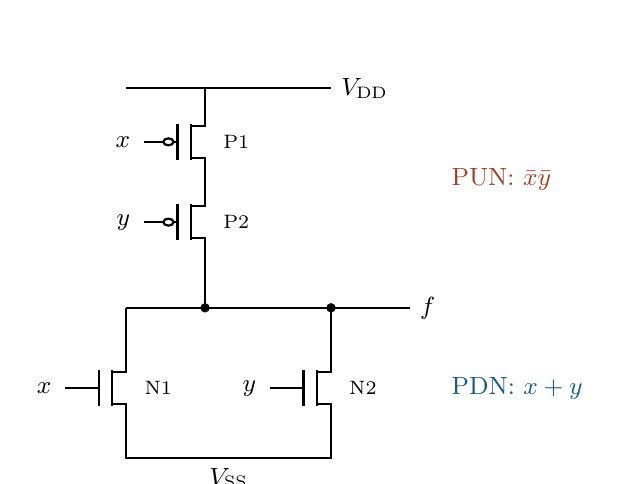
\begin{tikzpicture}[x=1cm,y=.68cm,line width=.8pt,font=\small]
 \MOS{P1}{0}{6.7}{x}{p}\MOS{P2}{0}{5.2}{y}{p}
 \MOS{N1}{-1}{2.1}{x}{n}\MOS{N2}{1.6}{2.1}{y}{n}
 \draw (-1,7.7)--(1.6,7.7) node[right] {$\VDD$};
 \draw (0,7.7)--(P1t) (P1b)--(P2t) (P2b)--(0,3.6);
 \draw (-1,3.6)--(2.6,3.6) node[right] {$f$};
 \draw (-1,3.6)--(N1t) (1.6,3.6)--(N2t);
 \draw (N1b)--(-1,.8)--(1.6,.8)--(N2b);
 \node[below] at (.3,.8) {$\VSS$};
 \fill (0,3.6) circle (1.7pt) (1.6,3.6) circle (1.7pt);
 \node[anchor=west,text=pcol] at (3,6) {PUN: $\bar x\bar y$};
 \node[anchor=west,text=ncol] at (3,2.1) {PDN: $x+y$};
\end{tikzpicture}
\end{center}
\begin{center}
\begin{tabular}{ccccc}\toprule
$x$&$y$&$w,z$&PDN on&$f$\\\midrule
0&0&any&0&1\\0&1&any&1&0\\1&0&any&1&0\\1&1&any&1&0\\\bottomrule
\end{tabular}
\end{center}
\answer{\textbf{Selected implementation: a 4T NOR.} Direct implementation of the
unsimplified expression uses five nMOS and five pMOS devices. The $wyz$ branch
is redundant; eliminating it preserves the function and saves six transistors.}

\newpage
\section*{1(b) Three-input minority function: 10T static CMOS}
The specified function is $f=\bar x\bar y+\bar x\bar z+\bar y\bar z$.
Complementing the function gives a PDN expression using only true input literals:
\begin{align*}
 \bar f&=(x+y)(x+z)(y+z)=xy+xz+yz\\
 &=xy+z(x+y),\\
 f&=\overline{xy+z(x+y)}
   =(\bar x+\bar y)(\bar z+\bar x\bar y).
\end{align*}
The left PDN branch has $x$ in series with $y$; the right branch has $z$ in series
with $(x\parallel y)$. The dual PUN has $(x\parallel y)$ in series with
$[z\parallel(x\text{ in series with }y)]$. All gates use true input literals.
\begin{center}
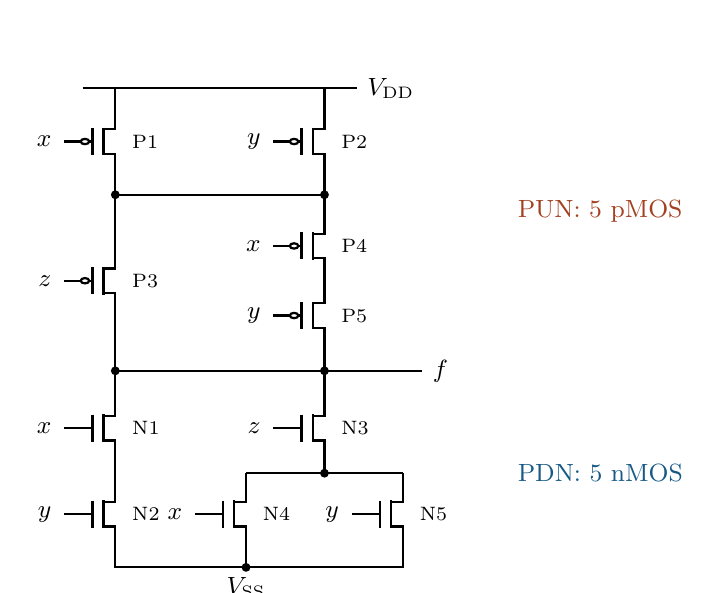
\begin{tikzpicture}[x=.83cm,y=.52cm,line width=.8pt,font=\small]
 \MOS{P1}{0}{10.7}{x}{p}\MOS{P2}{3.2}{10.7}{y}{p}
 \MOS{P3}{0}{7.3}{z}{p}\MOS{P4}{3.2}{8.15}{x}{p}\MOS{P5}{3.2}{6.45}{y}{p}
 \draw (-.5,12)--(3.7,12) node[right] {$\VDD$};
 \draw (0,12)--(P1t) (3.2,12)--(P2t);
 \draw (P1b)--(0,9.4)--(3.2,9.4)--(P2b);
 \draw (0,9.4)--(P3t) (3.2,9.4)--(P4t) (P4b)--(P5t);
 \draw (P3b)--(0,5.1)--(3.2,5.1)--(P5b);
 \draw (3.2,5.1)--(4.7,5.1) node[right] {$f$};
 \MOS{N1}{0}{3.7}{x}{n}\MOS{N2}{0}{1.6}{y}{n}
 \MOS{N3}{3.2}{3.7}{z}{n}\MOS{N4}{2}{1.6}{x}{n}\MOS{N5}{4.4}{1.6}{y}{n}
 \draw (0,5.1)--(N1t) (N1b)--(N2t);
 \draw (3.2,5.1)--(N3t) (N3b)--(3.2,2.6);
 \draw (2,2.6)--(4.4,2.6) (2,2.6)--(N4t) (4.4,2.6)--(N5t);
 \draw (N2b)--(0,.3)--(4.4,.3)--(N5b) (N4b)--(2,.3);
 \node[below] at (2,.3) {$\VSS$};
 \foreach \x/\y in {0/9.4,3.2/9.4,0/5.1,3.2/5.1,3.2/2.6,2/.3}
   \fill (\x,\y) circle (1.6pt);
 \node[anchor=west,text=pcol] at (6,9) {PUN: 5 pMOS};
 \node[anchor=west,text=ncol] at (6,2.6) {PDN: 5 nMOS};
\end{tikzpicture}
\end{center}
\begin{center}
\begin{tabular}{cccccc}\toprule
$x$&$y$&$z$&$xy+z(x+y)$&$f$&PUN on\\\midrule
0&0&0&0&1&1\\0&0&1&0&1&1\\0&1&0&0&1&1\\0&1&1&1&0&0\\
1&0&0&0&1&1\\1&0&1&1&0&0\\1&1&0&1&0&0\\1&1&1&1&0&0\\\bottomrule
\end{tabular}
\end{center}
\answer{\textbf{Total: 10T, with no input inverters.} The output is 1 exactly when
at most one input is 1. Both references use valid 12T networks; factoring the
function saves two transistors.}

\newpage
\section*{2. Four-way cyclic data selection using CMOS TGs}
Each specified control word has exactly one $c_j=1$. The design therefore assumes
\textbf{one-hot control}. Four transmission gates (TGs) select one data input for
each output:
\begin{align*}
z_3&=c_3a_3+c_2a_2+c_1a_1+c_0a_0,\\
z_2&=c_3a_2+c_2a_1+c_1a_0+c_0a_3,\\
z_1&=c_3a_1+c_2a_0+c_1a_3+c_0a_2,\\
z_0&=c_3a_0+c_2a_3+c_1a_2+c_0a_1.
\end{align*}
Equivalently, $z_i\leftarrow a_{(i+j-3)\bmod4}$ when $c_j=1$.
The next page shows all 16 TG data connections. The four complementary control
pairs $c_j,\bar c_j$ are shared across the circuit.

\subsection*{Transistor-level TG and complementary control}
\begin{center}
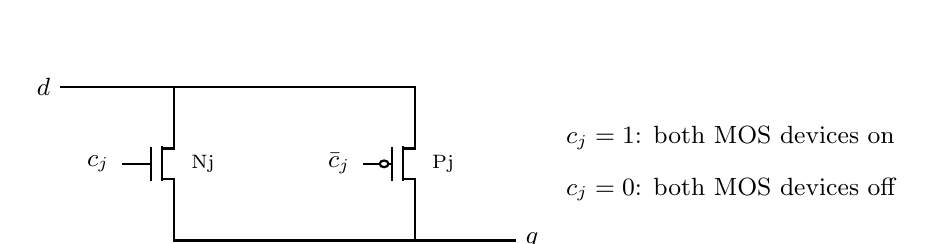
\begin{tikzpicture}[x=.85cm,y=.65cm,line width=.8pt,font=\small]
 \MOS{Nj}{0}{2.5}{c_j}{n}\MOS{Pj}{3.6}{2.5}{\bar c_j}{p}
 \draw (Njt)--(0,4)--(3.6,4)--(Pjt);
 \draw (Njb)--(0,1)--(3.6,1)--(Pjb);
 \draw (0,4)--(-1.7,4) node[left] {$d$};
 \draw (3.6,1)--(5.1,1) node[right] {$q$};
 \node[anchor=west] at (5.7,3) {$c_j=1$: both MOS devices on};
 \node[anchor=west] at (5.7,2) {$c_j=0$: both MOS devices off};
\end{tikzpicture}
\end{center}
The two MOS devices are \textbf{in parallel between the same data terminals}.
Unlike an nMOS-only pass gate, a CMOS TG passes both high and low logic levels
without a threshold-drop limitation. Its data path is bidirectional: the upper
and lower terminals in this drawing are data nodes, not supply rails. The bodies
still connect to $\VSS$ and $\VDD$, respectively.

\subsection*{Shared control inverters (four instances, $j=0,1,2,3$)}
\begin{center}
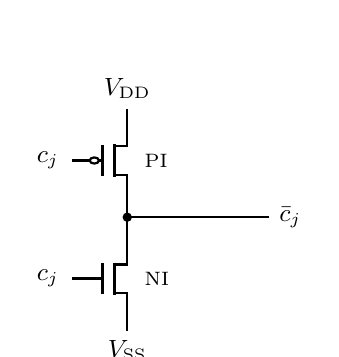
\begin{tikzpicture}[x=.9cm,y=.6cm,line width=.8pt,font=\small]
 \MOS{PI}{0}{4.7}{c_j}{p}\MOS{NI}{0}{2.2}{c_j}{n}
 \draw (PIt)--(0,5.8) node[above] {$\VDD$};
 \draw (PIb)--(0,3.5)--(NIt);
 \draw (0,3.5)--(2,3.5) node[right] {$\bar c_j$};
 \draw (NIb)--(0,1.1) node[below] {$\VSS$};
 \fill (0,3.5) circle (1.7pt);
\end{tikzpicture}
\end{center}
\answer{\textbf{Device count:} $16\text{ TGs}\times2+4\text{ inverters}\times2=40\text{T}$.
No output buffers are included. Only the four one-hot words are specified.
Zero selection leaves outputs floating; multiple selections can connect different
data sources together. The controller must maintain one-hot control and avoid
overlap during switching.}

\newpage
\section*{2. Complete TG connections and verification (continued)}
Each $\mathrm{TG}_j$ expands to the two MOS devices on the preceding page:
its nMOS gate connects to $c_j$ and its pMOS gate to $\bar c_j$.
All instances with the same control index share one inverter. Different output
buses are not connected to each other.
\begin{center}
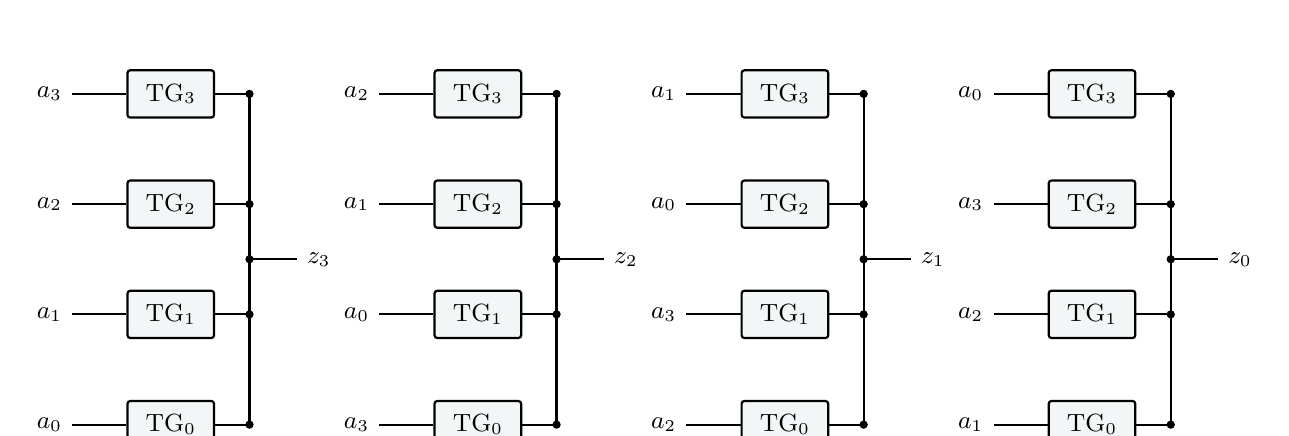
\begin{tikzpicture}[x=1cm,y=1cm,line width=.8pt,font=\small]
 \foreach \col/\zi in {0/3,1/2,2/1,3/0}{
   \begin{scope}[xshift=\col*3.9cm]
   \foreach \row/\cj in {0/3,1/2,2/1,3/0}{
     \pgfmathtruncatemacro{\ai}{mod(\zi+\cj+1,4)}
     \TG{tg\zi\cj}{1.25}{-\row*1.4}{\cj}
     \draw (0,-\row*1.4) node[left] {$a_{\ai}$}--(tg\zi\cj.west);
     \draw (tg\zi\cj.east)--(2.25,-\row*1.4);
     \fill (2.25,-\row*1.4) circle (1.5pt);
   }
   \draw (2.25,0)--(2.25,-4.2);
   \draw (2.25,-2.1)--(2.85,-2.1) node[right] {$z_{\zi}$};
   \fill (2.25,-2.1) circle (1.5pt);
   \end{scope}
 }
\end{tikzpicture}
\end{center}
\vspace{8pt}
\begin{center}
\begin{tabular}{ccccccccc}\toprule
$c_3$&$c_2$&$c_1$&$c_0$&Enabled TGs&$z_3$&$z_2$&$z_1$&$z_0$\\\midrule
1&0&0&0&All $\mathrm{TG}_3$&$a_3$&$a_2$&$a_1$&$a_0$\\
0&1&0&0&All $\mathrm{TG}_2$&$a_2$&$a_1$&$a_0$&$a_3$\\
0&0&1&0&All $\mathrm{TG}_1$&$a_1$&$a_0$&$a_3$&$a_2$\\
0&0&0&1&All $\mathrm{TG}_0$&$a_0$&$a_3$&$a_2$&$a_1$\\\bottomrule
\end{tabular}
\end{center}
\textbf{Example control word.} Set $c_2=1$ and all other controls to 0.
Only $\mathrm{TG}_2$ is enabled at each output. Tracing the connections gives
\[
 (z_3,z_2,z_1,z_0)=(a_2,a_1,a_0,a_3).
\]
The other three control words follow identically. The supplied Python checker
enumerates all four one-hot choices and all 16 data words, for $4\times16=64$
cases. It checks the expanded nMOS/pMOS connectivity as well as the equations.

\subsection*{If all control words must have defined outputs}
The 12 unspecified control words are outside this one-hot TG design's operating
condition. If the specification instead requires the AND-OR equations to hold for
arbitrary $c_0,\ldots,c_3$, use four NAND2 gates producing $\overline{c_j a_k}$
and one NAND4 per output. This requires $4\times4+8=24$T per output, or 96T in
total. It defines OR behavior for non-one-hot controls, at higher device cost
than the selector needed for the original four specified words.

\newpage
\section*{3(a) Logic function of the original pass-transistor circuit}
The upper nMOS is controlled by $A$ and passes $B$; the lower nMOS is controlled
by $\bar A$ and passes $\bar B$. Hence $F=B$ for $A=1$, and $F=\bar B$ for $A=0$:
\[
 \boxed{F(A,B)=AB+\bar A\bar B=\overline{A\oplus B}}\qquad\text{(XNOR)}.
\]
\begin{center}
\begin{tabular}{cccccc}\toprule
$A$&$B$&Enabled branch&Passed value&$F$&$\bar F$\\\midrule
0&0&Lower&$\bar B=1$&1&0\\0&1&Lower&$\bar B=0$&0&1\\
1&0&Upper&$B=0$&0&1\\1&1&Upper&$B=1$&1&0\\\bottomrule
\end{tabular}
\end{center}
This logic analysis treats the original devices as ideal switches. An nMOS-only
path can lose a threshold voltage when passing a high level; the original circuit
should not be described as a full-swing static CMOS output stage.

\section*{3(b) Complementary static CMOS XNOR}
For a static CMOS implementation, first write
\[
 \bar F=A\bar B+\bar A B=(A+B)(\bar A+\bar B).
\]
The PDN is $(A\parallel B)$ in series with $(\bar A\parallel\bar B)$.
Its dual PUN has two parallel branches: $A$ in series with $B$, and
$\bar A$ in series with $\bar B$.
\begin{center}
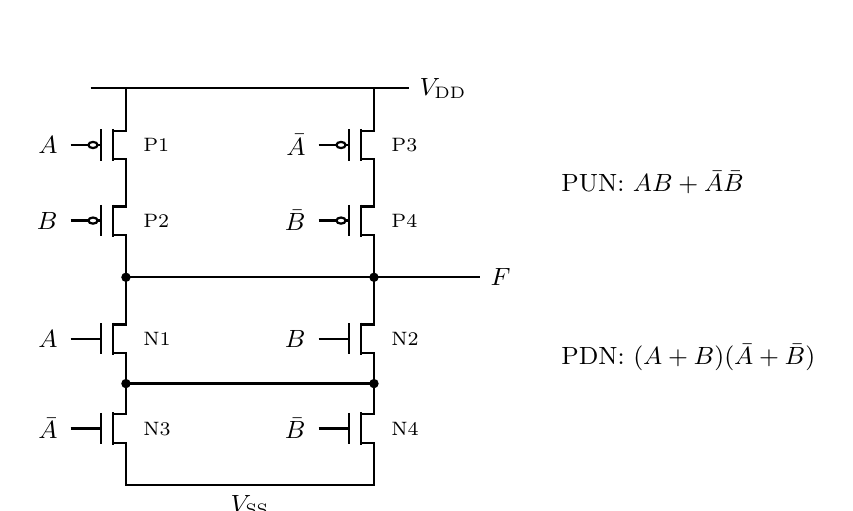
\begin{tikzpicture}[x=.9cm,y=.6cm,line width=.8pt,font=\small]
 \MOS{P1}{0}{7.3}{A}{p}\MOS{P2}{0}{5.7}{B}{p}
 \MOS{P3}{3.5}{7.3}{\bar A}{p}\MOS{P4}{3.5}{5.7}{\bar B}{p}
 \draw (-.5,8.5)--(4,8.5) node[right] {$\VDD$};
 \draw (0,8.5)--(P1t) (3.5,8.5)--(P3t) (P1b)--(P2t) (P3b)--(P4t);
 \draw (P2b)--(0,4.5)--(3.5,4.5)--(P4b);
 \draw (3.5,4.5)--(5,4.5) node[right] {$F$};
 \MOS{N1}{0}{3.2}{A}{n}\MOS{N2}{3.5}{3.2}{B}{n}
 \MOS{N3}{0}{1.3}{\bar A}{n}\MOS{N4}{3.5}{1.3}{\bar B}{n}
 \draw (0,4.5)--(N1t) (3.5,4.5)--(N2t);
 \draw (N1b)--(0,2.25)--(3.5,2.25)--(N2b);
 \draw (0,2.25)--(N3t) (3.5,2.25)--(N4t);
 \draw (N3b)--(0,.1)--(3.5,.1)--(N4b);
 \node[below] at (1.75,.1) {$\VSS$};
 \foreach \x/\y in {0/4.5,3.5/4.5,0/2.25,3.5/2.25}\fill (\x,\y) circle (1.7pt);
 \node[anchor=west] at (6,6.5) {PUN: $AB+\bar A\bar B$};
 \node[anchor=west] at (6,2.8) {PDN: $(A+B)(\bar A+\bar B)$};
\end{tikzpicture}
\end{center}
\answer{\textbf{8T core, or 12T including complementary-input generation.}
If $\bar A,\bar B$ are unavailable, add two 2T inverters of the form shown in
Problem 2, with inputs $A,B$, respectively. For every binary input word,
exactly one of the PUN and PDN conducts.}

\newpage
\section*{3(b) Optional 8T transmission-gate implementation}
A two-to-one CMOS TG selector implements the same function:
\begin{center}
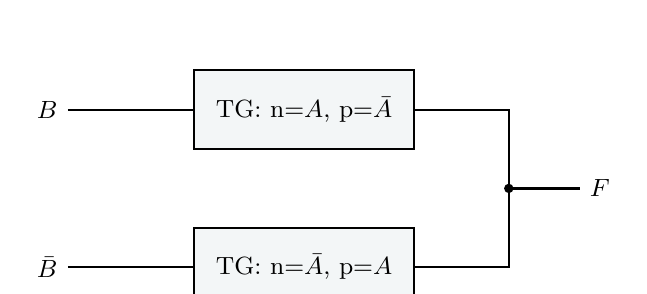
\begin{tikzpicture}[x=1cm,y=1cm,line width=.8pt,font=\small]
 \node[draw,minimum width=28mm,minimum height=10mm,fill=accent!5] (t1) at (0,0) {TG: n=$A$, p=$\bar A$};
 \node[draw,minimum width=28mm,minimum height=10mm,fill=accent!5] (t0) at (0,-2) {TG: n=$\bar A$, p=$A$};
 \draw (-3,0) node[left] {$B$}--(t1.west);
 \draw (-3,-2) node[left] {$\bar B$}--(t0.west);
 \draw (t1.east)--(2.6,0)--(2.6,-2)--(t0.east);
 \draw (2.6,-1)--(3.5,-1) node[right] {$F$};
 \fill (2.6,-1) circle (1.7pt);
\end{tikzpicture}
\end{center}
Each TG contains the two parallel MOS devices shown in Problem 2. Two TGs use
4T, and the two inverters generating $\bar A,\bar B$ use another 4T, for 8T total.
Only the upper path conducts for $A=1$; only the lower path conducts for $A=0$.
This mutually exclusive selection prevents $B$ and $\bar B$ from being connected
together. The primary answer remains the preceding static CMOS circuit because
it explicitly demonstrates complementary PUN/PDN construction.

\section*{Sources and method of comparison}
Original assignment: \texttt{homework1.pdf}, EE3032 Introduction to VLSI Design,
Fall 2024, one page. The following pre-existing handwritten documents
were supplied by the user. No author or license was identified. Their handwritten
content is not presented as newly authored work here.
\begin{itemize}
 \item \textbf{Reference A:} a user-supplied four-page HW1 correction/reference,
 including a cover. All solution content on pages 2--4 was reviewed.
 \item \textbf{Reference B:} a three-page student HW1 solution. All pages were reviewed.
\end{itemize}
The following comparison explains the independently selected corrections.

\newpage
\section*{Reference review and selection rationale}
\begin{tabular}{p{.09\linewidth}p{.39\linewidth}p{.43\linewidth}}\toprule
Problem&Reference review&Selected solution\\\midrule
1(a)&Both retain the unsimplified 10T network. A labels the redundant branch
with $\bar z$, contrary to the true-literal restriction; absorption makes this
branch irrelevant to the output.&
Read the original overbar correctly and simplify to $\overline{x+y}$: a 4T NOR.\\
1(b)&Both use valid 12T networks with PDN $(x+y)(x+z)(y+z)$.&
Preserve the minority function, factor the PDN as $xy+z(x+y)$, and use 10T.\\
2&Both have the correct cyclic selection wiring. B explicitly shows inverted
controls; A uses more abbreviated notation.&
Retain the valid wiring; expand the TG gate controls and shared inverters.
State the one-hot condition and the 40T count.\\
3&Both identify XNOR. A's complementary control bars can be distinguished, but
the upper MOS-type symbol is unclear. B's static CMOS structure is valid.&
Use the independently derived static CMOS circuit, consistent with B. Redraw
the complete TG alternative with explicit n/p controls; do not infer a wiring
error from A's ambiguous symbol.\\\bottomrule
\end{tabular}

\section*{Reproducible verification}
\texttt{verify\_logic.py} enumerates the input words and builds conducting graphs
from the MOS terminals in the diagrams: 16 cases for 1(a), 8 for 1(b), 64 specified
cases for 2, and 4 for each implementation of 3. It checks that static CMOS has
neither floating outputs nor rail shorts, and that each TG output reaches exactly
the selected data source. Inverter checks and unspecified-control examples bring
the total to 100 cases. These are ideal binary-switch checks, not HSPICE process,
delay, switching-transient, or analog-voltage simulations.
\end{document}
